% Chapter 1

\chapter{Problem Analysis} % Main chapter title

\label{Chapter2} % For referencing the chapter elsewhere, use \ref{Chapter1} 
In this chapter, the problem analysis as described by \citet{Prins2008} in Section \ref{BSD} will be applied. The problem owner will be described, a system description is given, stakeholder analysis is performed and a clear and concise problem definition is formulated. In the end, a research goal that fulfills the stakeholder and problem owner requirements is formulated.

\section{Problem owner analysis} \label{Problem owner analysis}
As mentioned in the previous section, this project is originated from Beenen. The higher management goal is to centralize maintenance support at a Beenen facility in Heerenveen or Zwolle. To accomplishing this goal, an implementation of CBM is desired and therefore have to be designed. Designing this tool requires analyzable data available from control systems and will be obtained in collaboration with Philips. Within Beenen, several employees are connected to the installations at Philips Drachten by providing maintenance support and services. Thom Verwater and Kevin Schipper are the leading R\&D employees aiming for an implementation of CBM to their designed installations and can therefore be seen as the problem owners. 

The maintenance department of Philips will play a big role during this design project. The aimed application of CBM to their RACs will contribute to their objectives, stated in Section \ref{Problem Context}, as well. However, Philips will not be seen as problem owner since the intended output of this design project will be property of Beenen. 

\section{System description} \label{System description}
The initial goal of the problem owners is to design a system that is able to predict upcoming maintenance by analyzing data that is available from their designed control systems. This tool should then be added to the products and services Beenen offers. It indicates that the investigated system is a maintenance decision making system that consist of input, output, external factors and subsystems. Focusing on the Philips case, data, such as currents, torques, temperatures and positions errors, available from the RACs can then be seen as the input for the maintenance system and a maintenance schedule as the output. Subsystems within the boundaries of the system are the functions: data logging, comparing limit values and schedule compiling. Activities as performing maintenance and ordering inventory are outside the scope of this project and are therefore not within the boundaries of the described system. A diagram of the system description with corresponding input, output and subsystems can be seen in Figure \ref{fig:System_Description}. 
\begin{figure}[ht]
\centering
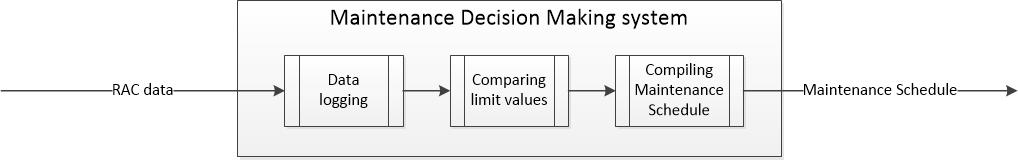
\includegraphics[width=\textwidth]{Figures/Intended_System_Description}
\caption[General system description]{A general system description with corresponding input, output and subsystems.}
\label{fig:System_Description}
\end{figure} 

Applying CBM to all installations at Philips Drachten will be an extensive and complex task. Executing such a project is therefore not realistic in the available time for this project. Therefore, this project focuses on one specific RAC only. Implementing the design on the control system of the RAC is done by software engineers at Beenen and therefore outside the system-boundaries of this project. 

However, it would be possible to shift the boundaries and expand the number of RACs. The number of maintenance actions, feasibility, and related maintenance costs are examples of performance indicators that determine the appropriateness of applying CBM to a specific cell. This indicators are judged by Philips employees that have experience with the installations.

This system description is generic written because the aimed CBM tool as described in Section \ref{Business context} should be applied to all control systems Beenen designs or maintains, in the end. Nevertheless, from interviews with members of the OG and OTD it is discussed to focus this design project on RAC RB34. One of the Robot Arms within this cell leaks some oil and upcoming maintenance is expected, therefore it is suitable to investigate the data regarding this cell. A description of this cell is given in Section \ref{RB34 description} and the entire process description (dutch) can be found in Appendix \ref{AppendixA}. 

\subsection{Description of RAC RB34} \label{RB34 description}
RB34 is part of AL SUA3 that assembles the shaver unit of mini-company Thor, the 3000 series shaver. Other RACs that are part of SUA3 are RB31, RB32, RB33, RB35 and TF135. Where the RB cells are all responsible for assembling a different part of the shaver unit from the 3000 series and the TF cell is responsible for feeding trays to RB35 carrying parts that are assembled to the shaver unit. A double conveyor belt ensures a continuous flow of product carriers, in deutsch: Werk Trägers (WT)s and in dutch: productdragers, that support the assembly objects. 

Firstly, the assembly objects arrive in RB34 on WTs from RB33 at the first position and Robot Arm 1, a Adept Cobra\textsuperscript{\tiny{TM}} s600, assembles the holder springs, see Figure \ref{fig:Holder springs}, to the assembly object. Thereafter, the WT moves to the second position in RB34 and Robot Arm 2, also a Cobra s600, assembles the Holders, see Figure \ref{fig:Holders}. The holder springs and Holders are equal for every shaver unit of Thor. Via a sensor, the presence of a holder spring and a WT at position 1 or 2 is detected. Additional, a scrap cutter, in dutch: schrot snijder, with conveyor belt provides the Holder Springs to Robot Arm 1.

\begin{figure}[ht]
\centering
\begin{subfigure}[b]{0.49\textwidth}
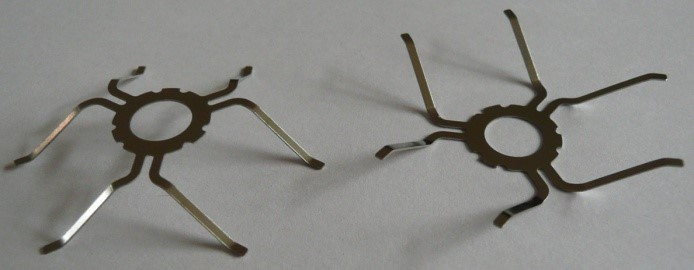
\includegraphics[width=\textwidth, height=3cm]{Figures/Afbeeldin1_Holder_springs}
\caption{Holder springs}
\label{fig:Holder springs}
\end{subfigure}
\begin{subfigure}[b]{0.49\textwidth}
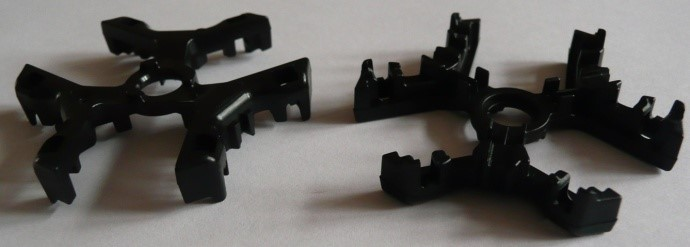
\includegraphics[width=\textwidth, height=3cm]{Figures/Afbeelding2_Holders}
\caption{Holders}
\label{fig:Holders}
\end{subfigure}
\caption[Holder Springs and Holders that are assembled by RB34]{Holder Springs and Holders that are assembled by RB34}
\label{fig:Holders_Holder springs}
\end{figure}

RACs are highly automated and require minimal human supervision during normal operation. In Figure \ref{fig:RACmodel}, it can be seen what inputs and outputs are of a RAC \parencite{Mohamed2001} in the current situation. Inputs are the above described WTs carrying the assembly objects with additional production orders, other inputs are sensors that can detect the holders and springs, spare parts that are necessary during maintenance, programs that control the RAC and tools and fixtures such as the robot arms and feeders. Output of the RAC are the finished products that are transported by conveyor belts to the next RAC where another part of the shaver unit is assembled. Furthermore, feedback on the activities is given by the control system that is integrated to the computer of the RAC in the form of data files. The types of data that are available will be described in Section \ref{Data Gathering}. In the current situation, limit values are not known and therefore it is impossible to determine on forehand which RACs require maintenance according to the data files.
\begin{figure}[ht]
\centering
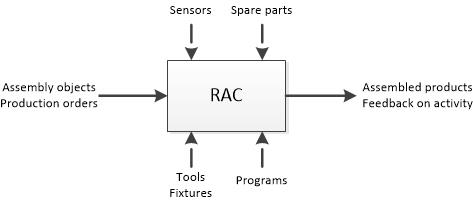
\includegraphics[width=0.7\textwidth]{Figures/RACmodel}
\caption[Model of an RAC]{Model of an RAC}
\label{fig:RACmodel}
\end{figure}

\section{Stakeholder analysis} \label{Stakeholder analysis}
For this design project several stakeholders can be reviewed. The problem owners, Thom Verwater and Kevin Schipper, are the main stakeholders since they want to implement the intended design of this project for their products and services. Those two engineers from Beenen are representing the company and therefore Beenen itself or the director is not be reviewed as stakeholder. Furthermore, the higher management goal of the problem owners is to centralize the maintenance for their customers. In other words, the goal is to generate maintenance schedules at Beenen Heerenveen instead of on-site with live data from the control systems at customers. By scheduling all predictable maintenance for customers a more efficient maintenance system can be obtained. Centralizing all maintenance activities for multiple customers is an extensive task and is not realistic for the time of this project. Therefore, this project focuses on ALs and RACs within mini-company Thor of Phililps Drachten, as mentioned in Section \ref{Business context}.

The maintenance department of Philips Drachten, in particular Maintenance Engineer Dirk Jan Dunsbergen, can also be seen as stakeholder. The project focuses on shaver RACs at Philips and a CBM tool will be designed for these installations. An effective result of this project that can be implemented to these systems will most likely result in a decreasing downtime of the RACs, increasing the throughput-rate of the entire mini-company. Philips Drachten as a company is not reviewed as stakeholder, the same reasoning as applied to Beenen as stakeholder can be applied here. 

A Support Group, in dutch: Ondersteunende Groep (OG), is assigned to one or more mini-companies and consist of the following managers and engineers: Maintenance Engineer, Production Manager, Assistant Production Manager, Quality Manager and Technical Support Mechanic. All of the managers and engineers within this OG are open for questions regarding quality and production of products. However, for this design project, most of them are not of importance since they are not related directly to the maintenance decision making process. Members of the Maintenance Technical Support, in dutch: Onderhoud Technische Dienst (OTD), are responsible for the physical maintenance and repair of RACs and other installations at the AL. Communication with the OTD goes via the Line Mechanic who has a leading function within the OTD and therefore the regular mechanics are not considered as stakeholders. A description of all employees, that are of importance to this project, with corresponding activities and stakes in this project are listed in Table \ref{tab:philips employees}. 

\begin{center}
\begin{longtable}[width=\textwidth]{ p{0.18\textwidth} | p{0.76\textwidth}}
\caption[Stakeholders]{Stakeholders} \vspace{0.3cm} \label{tab:philips employees} \\
Function & Activity/Stake \\ [1ex]
\hline \\
\parbox[t]{0.15\textwidth}{R\&D\\Engineer\\(Beenen)} & Responsible for the R\&D department at Beenen Heerenveen and also the problem owner for this project, see Section \ref{Problem owner analysis} . Strive to improve and develop existing and new products, machines and systems. Furthermore, ensuring smooth transfer of new technologies to other groups within Beenen. By supervising this design project and building further on the aimed CBM tool, the R\&D engineer benefits from this project. \\ [2ex]
\parbox[t]{0.15\textwidth}{Software\\Engineer\\(Beenen)} & Software engineers at Beenen are responsible for development of networks, operating systems, databases and applications. Control systems designed and installed by Beenen need integration of these components. Frank Velthuis is a software engineer working for Beenen at Philips. He is responsible for maintaining and updating the software installed on the RACs. His knowledge can be useful to provide communicating networks between RACs and a higher level system where all available information and data can be combined and processed. Furthermore, the desired CBM tool should be designed partially and integrated in the higher level system by a software engineer. \\ [2ex]
\parbox[t]{0.15\textwidth}{Maintenance\\Engineer\\(Philips)} & Responsible for continuous running of equipment and machinery. Focuses on minimizing downtime by preventing breakdowns and failures. By applying CBM, he aims to reduce the unplanned downtime of all RACs. Conclusions resulting from this project are reviewed and eventually implemented by him. The Maintenance Engineer works closely together with the researcher in order to provide all information regarding maintenance that is necessary to execute the project.  \\ [2ex]
\parbox[t]{0.15\textwidth}{Technical\\Support\\Group\\(Philips)} & Responsible for technical support and problem-shooting for ALs. Focuses on adequate and solid repair of equipment and installations. Works together with software engineers to maintain the systems and keep production running. His knowledge about operating systems can be helpful for the researcher to understand how data available from the RAC can be obtained.\\ [2ex]
\parbox[t]{0.15\textwidth}{Line\\Mechanic\\(Philips)} & Responsible for physical maintaining the production process by ensuring operation of machinery and mechanical equipment. His knowledge about robot arms and other equipment is necessary to determine what maintenance can be predictable. Furthermore, the tasks of the line mechanic can be influenced by implementation of a CBM tool.   \\
\end{longtable}
\end{center}

Stakeholders such as customers of Beenen that are offered installation systems where this design is implemented will not be seen as stakeholders for this project. This is because the stake of those customers correspond to the same objective Beenen has and is not adding extra requirements to the design.

Employees of Beenen that work with the maintenance system can also be considered as stakeholders. Firstly, software engineers need the skills to be able to apply the intended result of this project to their existing products and services. Secondly, other maintenance employees, mechanics and technicians, have to interpret results from the newly designed maintenance system tool in order to perform maintenance. 

\section{Problem definition} \label{Problem definition}
Maintenance performed by Beenen on equipment of customers is handled differently per customer. As mentioned before, this project is a collaboration with Philips and therefore, this project only focuses on the maintenance there. Beenen has a service contract with Philips regarding the software installed on the RACs and ALs. In contrast to other companies, the service contract with respect to Philips state that Beenen is responsible for providing only software support for these ALs. Physical support and maintenance is performed by the OTD of Philips.  

The problem owners, Thom and Kevin from Beenen, want to implement a CBM tool to their products and services to solve the problem of scheduling maintenance for all customers. In the system description this objective is scoped down to the maintenance system at Philips. From this system description it can be concluded that the problem is functional because the problem lays at the output of the system, a lacking maintenance schedule. This schedule is lacking since there is nothing monitored about the condition or average lifetime of the equipment. In this way, it is very hard to predict or prevent upcoming maintenance resulting in unnecessary downtime and high maintenance cost. This makes the problem functional and realistic and therefore the BSD method is applicable to this research project.

The problem statement that can be derived from the information provided by the management and the information stated above and in the previous sections of this chapter is:
\begin{center}
\textit{The use of corrective maintenance to RACs at Philips Drachten causes unplanned downtime, resulting in lower availability of machines than desired.}\\
\end{center}

\section{Design goal} \label{Design goal}
As discussed in Section \ref{Business context} and the previous sections from this chapter, the initial goal of the problem owners is to provide CBM to their designed control systems, helping Beenen to centralize maintenance support. By zooming in to RAC RB34 at Philips a more detailed system description can be provided and a clear and concise goal can be formulated. From this, the design goal of this project can be stated as follows:
\begin{center}
\textit{Improve the maintenance schedule at Philips Drachten for RAC RB34 by designing a CBM tool that satisfies the maintenance requirements and helps Beenen B.V. centralizing maintenance.}\\
\end{center}


%\parencite{Wieringa2014}
%Knowledge questions:\\
%What effects are produced by the interaction between artifact and context?\\
%Do the effects satisfy requirements?
